% Scalar instruction entry source: tools/generate_scalar_instruction_catalog.py.
\subsection{\texttt{FENCE.I}}
\label{sec:scalar-fence_i}
\index{FENCE.I@\texttt{FENCE.I}}
\begin{sloppypar}\noindent\textbf{Purpose.} Synchronizes instruction fetch with prior stores to instruction memory for the current execution context.\end{sloppypar}\smallskip
\noindent\textbf{Syntax.}\par
\begin{lstlisting}[style=ptoscalarcode]
fence.i
\end{lstlisting}
\noindent\textbf{Encoding.}\par
\noindent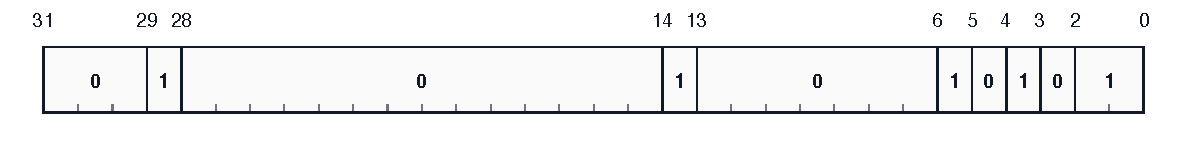
\includegraphics[width=\textwidth]{figs/encoding/scalar_instruction_entries/enc_fence_i.pdf}\par\smallskip
\begin{description}[leftmargin=0.18\linewidth,style=nextline]
\item[Format] \texttt{L32} \texttt{32-bit} scalar word.
\item[Pattern] \texttt{00010000000000000010000000101011}.
\end{description}
\noindent\textbf{Classification.}\par
\begin{description}[leftmargin=0.18\linewidth,style=nextline]
\item[Category] System, Cache, SSR, and Execution Control.
\item[Family] Execution Control.
\item[Execution class] \texttt{SYS}; uop\_kind=SYS.
\end{description}
\noindent\textbf{Operand fields.}\par
\noindent No variable operand fields are present in this fixed encoding.\par\smallskip
\noindent\textbf{Operation.}\par
\begin{lstlisting}[style=ptoscalarcode]
FenceI()  // instruction-cache fence
\end{lstlisting}
\Needspace{0.08\textheight}
